%!TEX program = xelatex
\documentclass[cn,hazy,pku,12pt,normal,math=newtx,cite=super]{elegantnote}
\title{Fe(OH)$_3$溶胶的制备与性质研究}

\author{刘松瑞 \quad 2100011819 \\ 组号:24 \quad 组内编号:5 \quad 合作者:万乘}
\institute{化学与分子工程学院}

\expdate{\zhdate{2023/10/25}}
\temperature{21.25 \si{^{\circ}C}}
\pressure{101.74 \si{kPa}}

\usepackage{gensymb}
\usepackage{array}
\usepackage{subfigure}
\usepackage[fontset=windows]{ctex}
\usepackage{graphicx}
\usepackage{float}
\usepackage{caption}
\usepackage{multirow}
%\usepackage{subfig}
%\usepackage{float}
\begin{document}

\maketitle

\keywords{氢氧化铁溶胶 \quad 电导 \quad 聚沉 \quad 电泳 \quad $\zeta$电势}

\abstracts{
    本次实验中,首先通过水解 $\rm FeCl_3$ 制备 $\rm Fe(OH)_3$ 溶胶,然后使用透析法纯化溶胶至符合电泳的电导率要求
    。然后使用电泳法实验测定 $\rm Fe(OH)_3$ 溶胶的 $\zeta$ 电势,但是与文献值对比存在较大误差,产生误差的原因
    可能有:界面清晰度较差,第二次测量吸出了一定量辅助液-胶体混合物,电泳时温度、浓度与 pH 值的影响等等。
    
}

\newpage


\section{引言}

\subsection{实验目的与原理}

实验目的与原理详见预习报告图~\ref{1}。 \cite{pcl2002}

\begin{figure}[htbp]
    \centering
    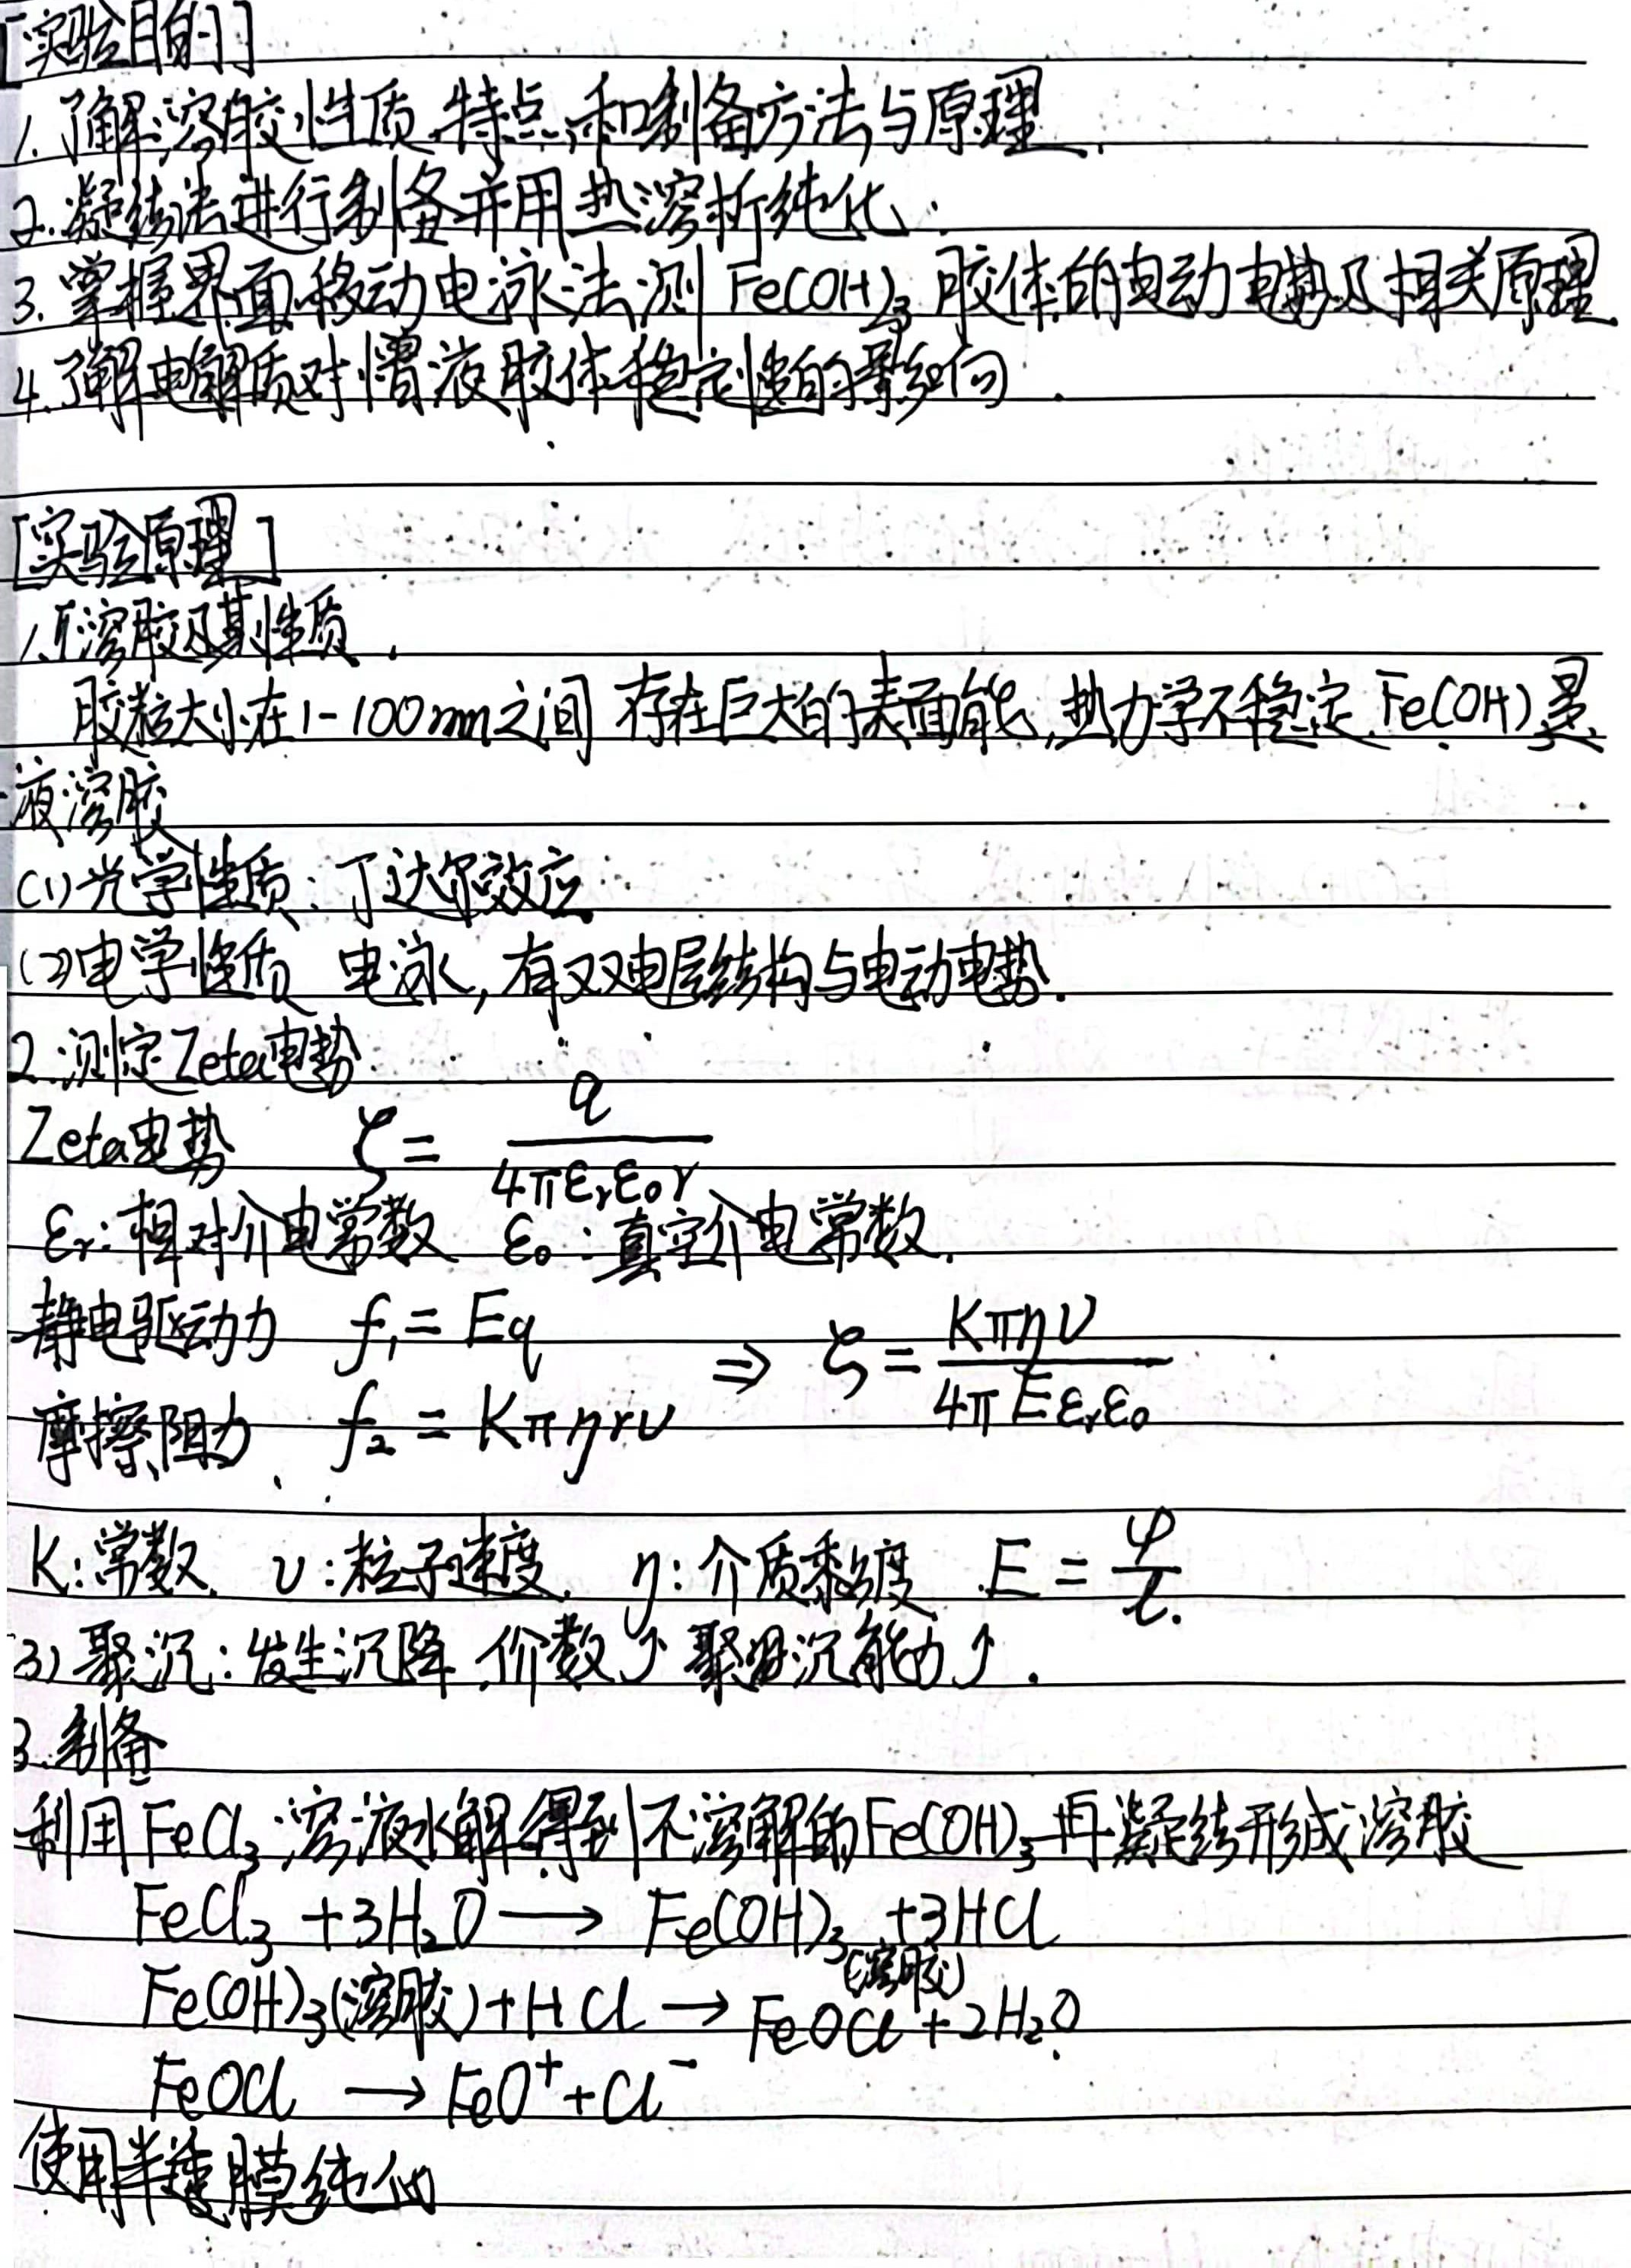
\includegraphics[width = .70\textwidth]{image/yxbg_1.jpg}
    \caption{实验的目的与原理}\label{1}
\end{figure}

\subsection{实验方法}

制备并纯化 $\rm Fe(OH)_3$ 胶体,并使用上一组同学制备的 $\rm Fe(OH)_3$ 胶体进行电泳实验。

\section{实验部分}

\subsection{实验步骤}

实验步骤详见预习报告图~\ref{b} 与图~\ref{4} 。
\begin{figure}[htbp]
    \centering
    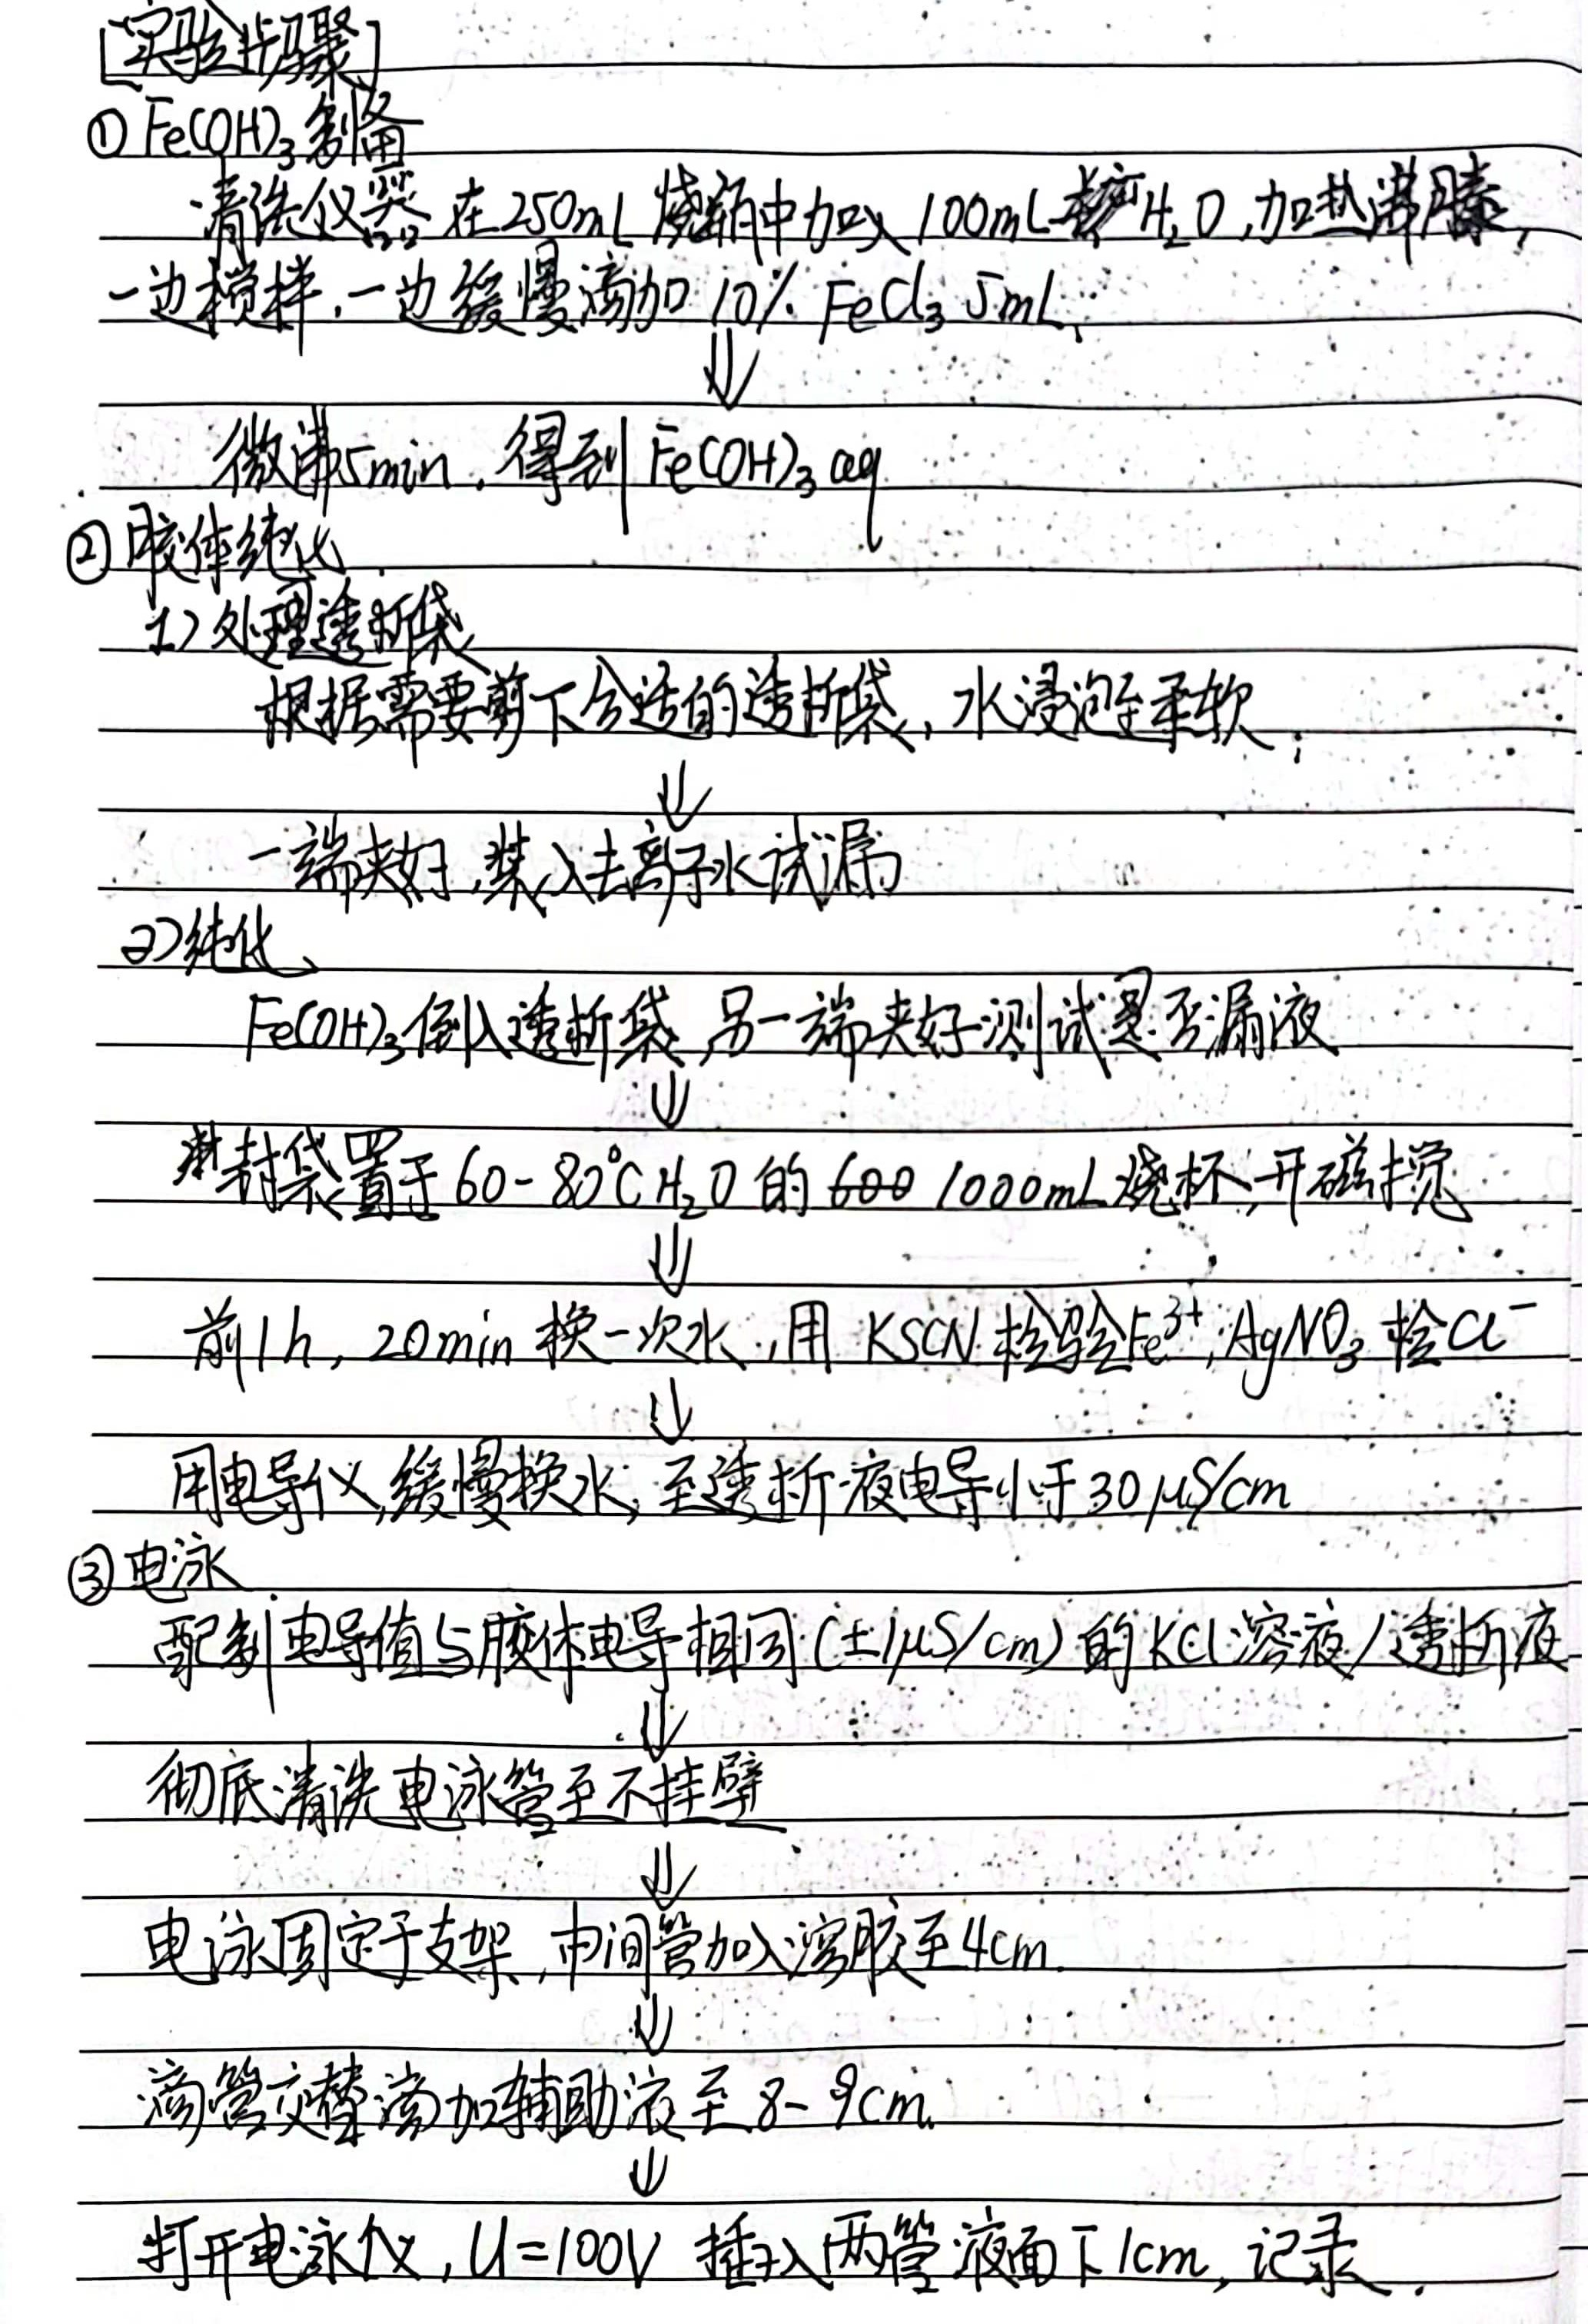
\includegraphics[width = .70\textwidth]{image/yxbg_2.jpg}
    \caption{实验步骤}\label{b}
\end{figure}

\begin{figure}[htbp]
    \centering
    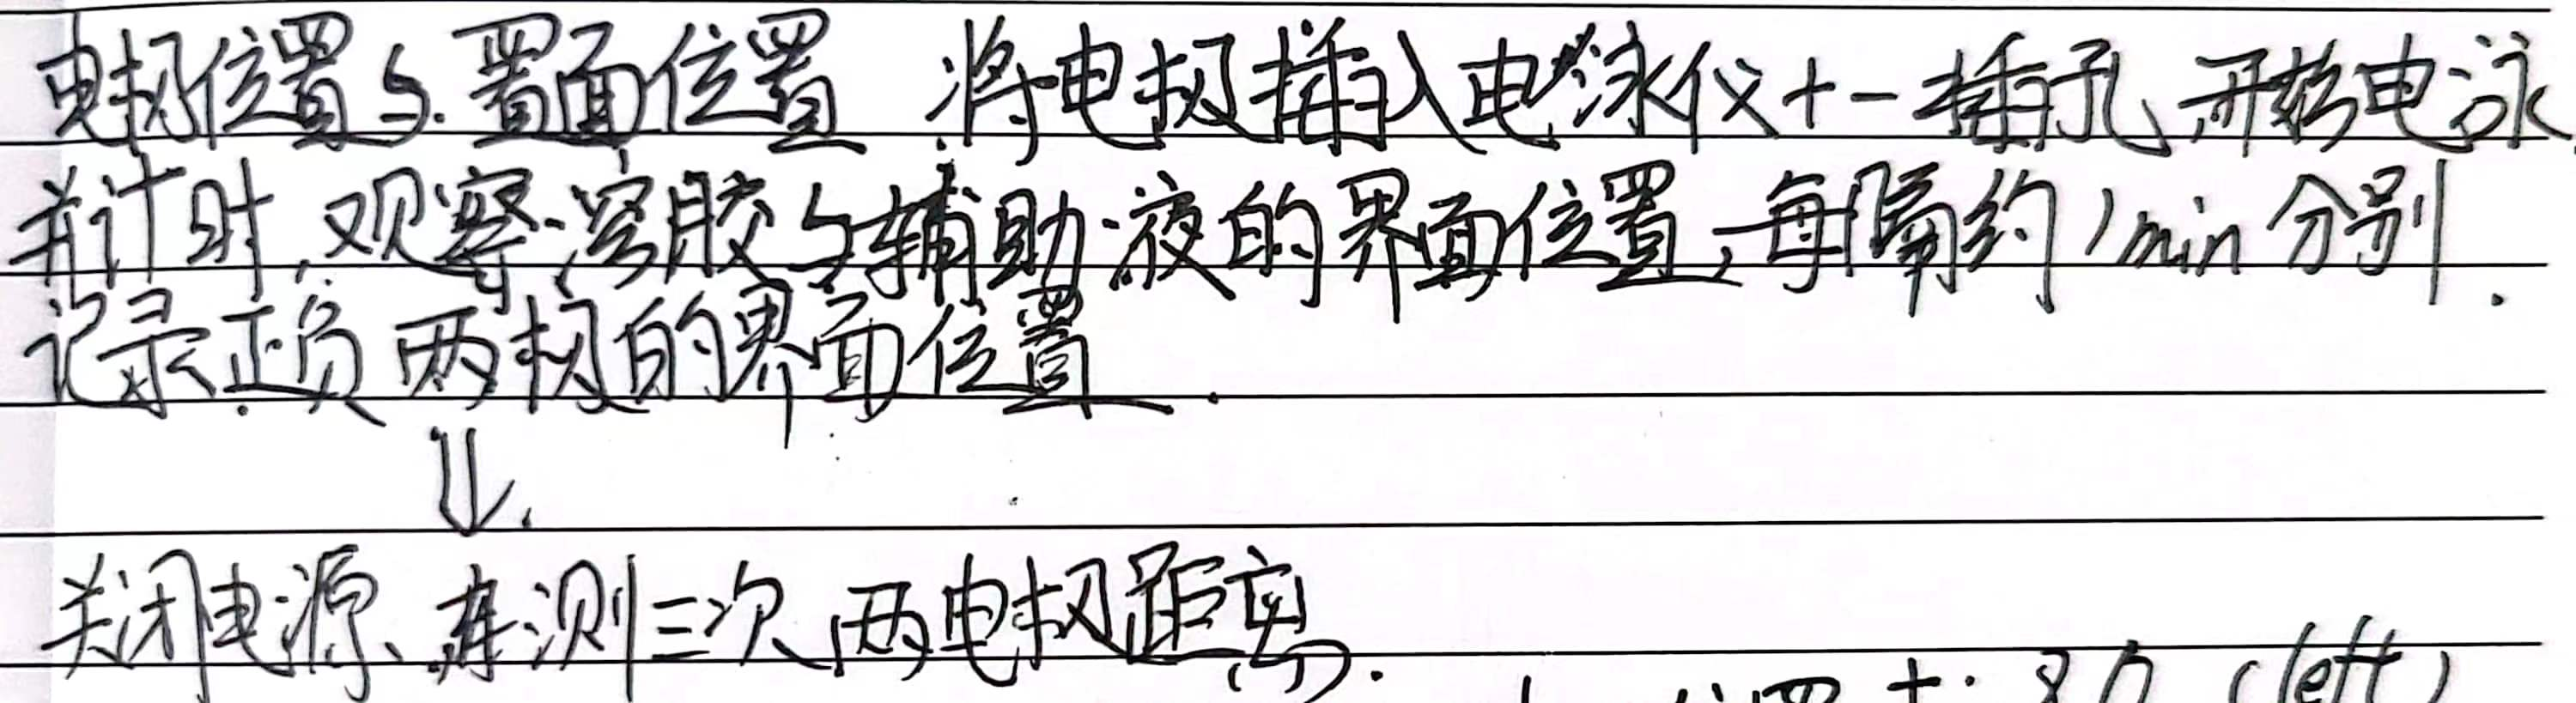
\includegraphics[width = .70\textwidth]{image/yxbg_3.jpg}
    \caption{实验步骤(续)}\label{4}
\end{figure}

\newpage

\subsection{仪器与药品}

\begin{enumerate} %有序列表
    \item 试剂 \\   10\% $\rm FeCl_3$ 溶液,
                    0.01 $\rm mol \cdot L^{-1}$ $\rm AgNO_3$ 溶液,
                    0.1 $\rm mol \cdot L^{-1}$ KSCN 溶液,
                    0.08 $\rm mol \cdot L^{-1}$ KCl 溶液,
                    尿素。
    \item 仪器 \\ 滴管,单口烧瓶,烧杯,试管,5 mL 量筒,透析袋,透析袋夹子;电加热套,电磁
    搅拌器,电导率仪,U 形电泳管,稳压电泳仪,铂电极,水浴锅,秒表,电子天平。
\end{enumerate}

\section{实验现象与数据处理}

\subsection[short]{$\rm Fe(OH)_3$溶胶的制备与纯化}

在煮沸的去离子水中滴加 $\rm FeCl_3$ 得到红棕色 $\rm Fe(OH)_3$ 溶胶后,对其进行透析纯化。
透析过程中,每间隔一定时间更换一次水,并用试剂检测透析液中的残余离子或用电导率仪测量透析液和溶胶的电导率,相关数据记录于表 \ref{5} 中。

\begin{table}[h]
    \centering
    \caption{溶胶的热透析数据}
    \label{5}
    \begin{tabular}{cccccc}
    \hline
    次数 & t/min & $\rm Fe^{3+}$ & $\rm Cl^-$ & 透析液电导率/ $\rm \mu S \cdot   cm^{-1}$ & 溶胶电导率/ $\rm \mu S \cdot   cm^{-1}$ \\ \hline
    0 & 0   & - & + & --            & --    \\
    1 & 17  & - & + & --            & --    \\
    2 & 54  & - & + & --            & --    \\
    3 & 82  & - & + & --            & --    \\
    4 & 100 & - & + & --            & --    \\
    5 & 122 & - & + & 24.9          & --    \\
    6 & 150 & - & + & $<$30           & --    \\
    7 & 194 & - & + & $<$20           & --    \\
    8 & 216 & - & - & --            & 156.9 \\ \hline
    \end{tabular}
\end{table}

表中 $\rm Fe^{3+}$ 与 $\rm Cl^-$ 两列,+ 表明滴加 KSCN 溶液或 $\rm AgNO_3$ 溶液有沉淀析出
,- 表示无沉淀析出。由于使用的透析袋过于陈旧,出现很多破损与漏液现象。因此在第五次换水后,我们更换了透析袋。
由于透析过程中,透析液的电导率在时刻地变化,因此在第六组之后仅描述一个大致的范围.
在经过 216 分钟透析后,得到溶胶电导率为 156.9 $\rm \mu S \cdot cm^{-1}$ 的红棕色 $\rm Fe(OH)_3$ 溶胶

\subsection[short]{测量$\rm Fe(OH)_3$溶胶的$\zeta$电势}

测量待测溶胶的电导率为 25.6 $\rm \mu S \cdot cm^{-1}$,为使得其液面更加清晰,向溶液中加入 0.98 g 尿素。
在加入尿素后,可能是由于加入过程中引入了电解质杂质,溶胶发生了聚沉,产生大量絮状沉淀,无法继续实验。
更换溶胶,测量待测溶胶的电导率为 20.5 $\rm \mu S \cdot cm^{-1}$,配置电导率为 20.8 $\rm \mu S \cdot cm^{-1}$
的 KCl 溶液辅助液,未加入尿素。

在第一次测定时,由于加入辅助液速度过快与未使用尿素保护等原因,使得胶体界面模糊无法进行读数。
吸出一定量辅助液-胶体混合物,再小心地滴加辅助液,进行第二次测量。由于界面清晰度依旧有限,测量的数据
仅保留两位有效数字。测得电极位置 $h_{(-)} = 7.90\ {\rm cm}$,$h_{(+)} = 8.00\ {\rm cm}$。
用软尺测量两电极之间的距离,如下表 \ref{a} 所示。可得 $\overline{l} = 22.84 {\rm cm}$,$\sigma_l = 0.09 {\rm cm}$。
因此得到电极间的距离为 $(22.84 \pm 0.09)$ cm。

\begin{table}[h]
    \centering
    \caption{电极间距离测量数据}
    \label{a}
    \begin{tabular}{cc}
    \hline
    次数 & $l$/cm  \\ \hline
    1  & 22.87 \\
    2  & 22.90 \\
    3  & 22.74 \\ \hline
    \end{tabular}
\end{table}

电泳时两极间电势差恒定为 103 V,电泳实验结果如下表 \ref{6} 所示。

\begin{table}[h]
    \centering
    \caption{溶胶电泳速率测定数据}
    \label{6}
    \begin{tabular}{ccccc}
    \hline
    t/min & $h_{(-)} /{\rm cm}$ & $\Delta h_{(-)} /{\rm cm}$ & $h_{(+)} /{\rm cm}$ & $\Delta h_{(+)} /{\rm cm}$ \\ \hline
    0     & 3.8           & 0.0                  & 3.8           & 0.0                  \\
    1     & 4.0           & 0.2                  & 3.5           & 0.3                  \\
    2     & 4.2           & 0.4                  & 3.4           & 0.4                  \\
    3     & 4.3           & 0.5                  & 3.1           & 0.7                  \\
    4     & 4.5           & 0.7                  & 3.0           & 0.8                  \\
    5     & 4.5           & 0.7                  & 2.8           & 1.0                  \\
    6     & 4.7           & 0.9                  & 2.6           & 1.2                  \\
    7     & 4.8           & 1.0                  & 2.5           & 1.3                  \\
    8     & 4.9           & 1.1                  & 2.3           & 1.5                  \\
    9     & 5.0           & 1.2                  & 2.1           & 1.7                  \\ \hline
    \end{tabular}
\end{table}

利用如上数据,作$\Delta h_{(-)} - t$图与$\Delta h_{(+)} - t$图,并对其进行线性回归,如下图 \ref{7} 所示
\begin{figure}[htbp]
    \centering
    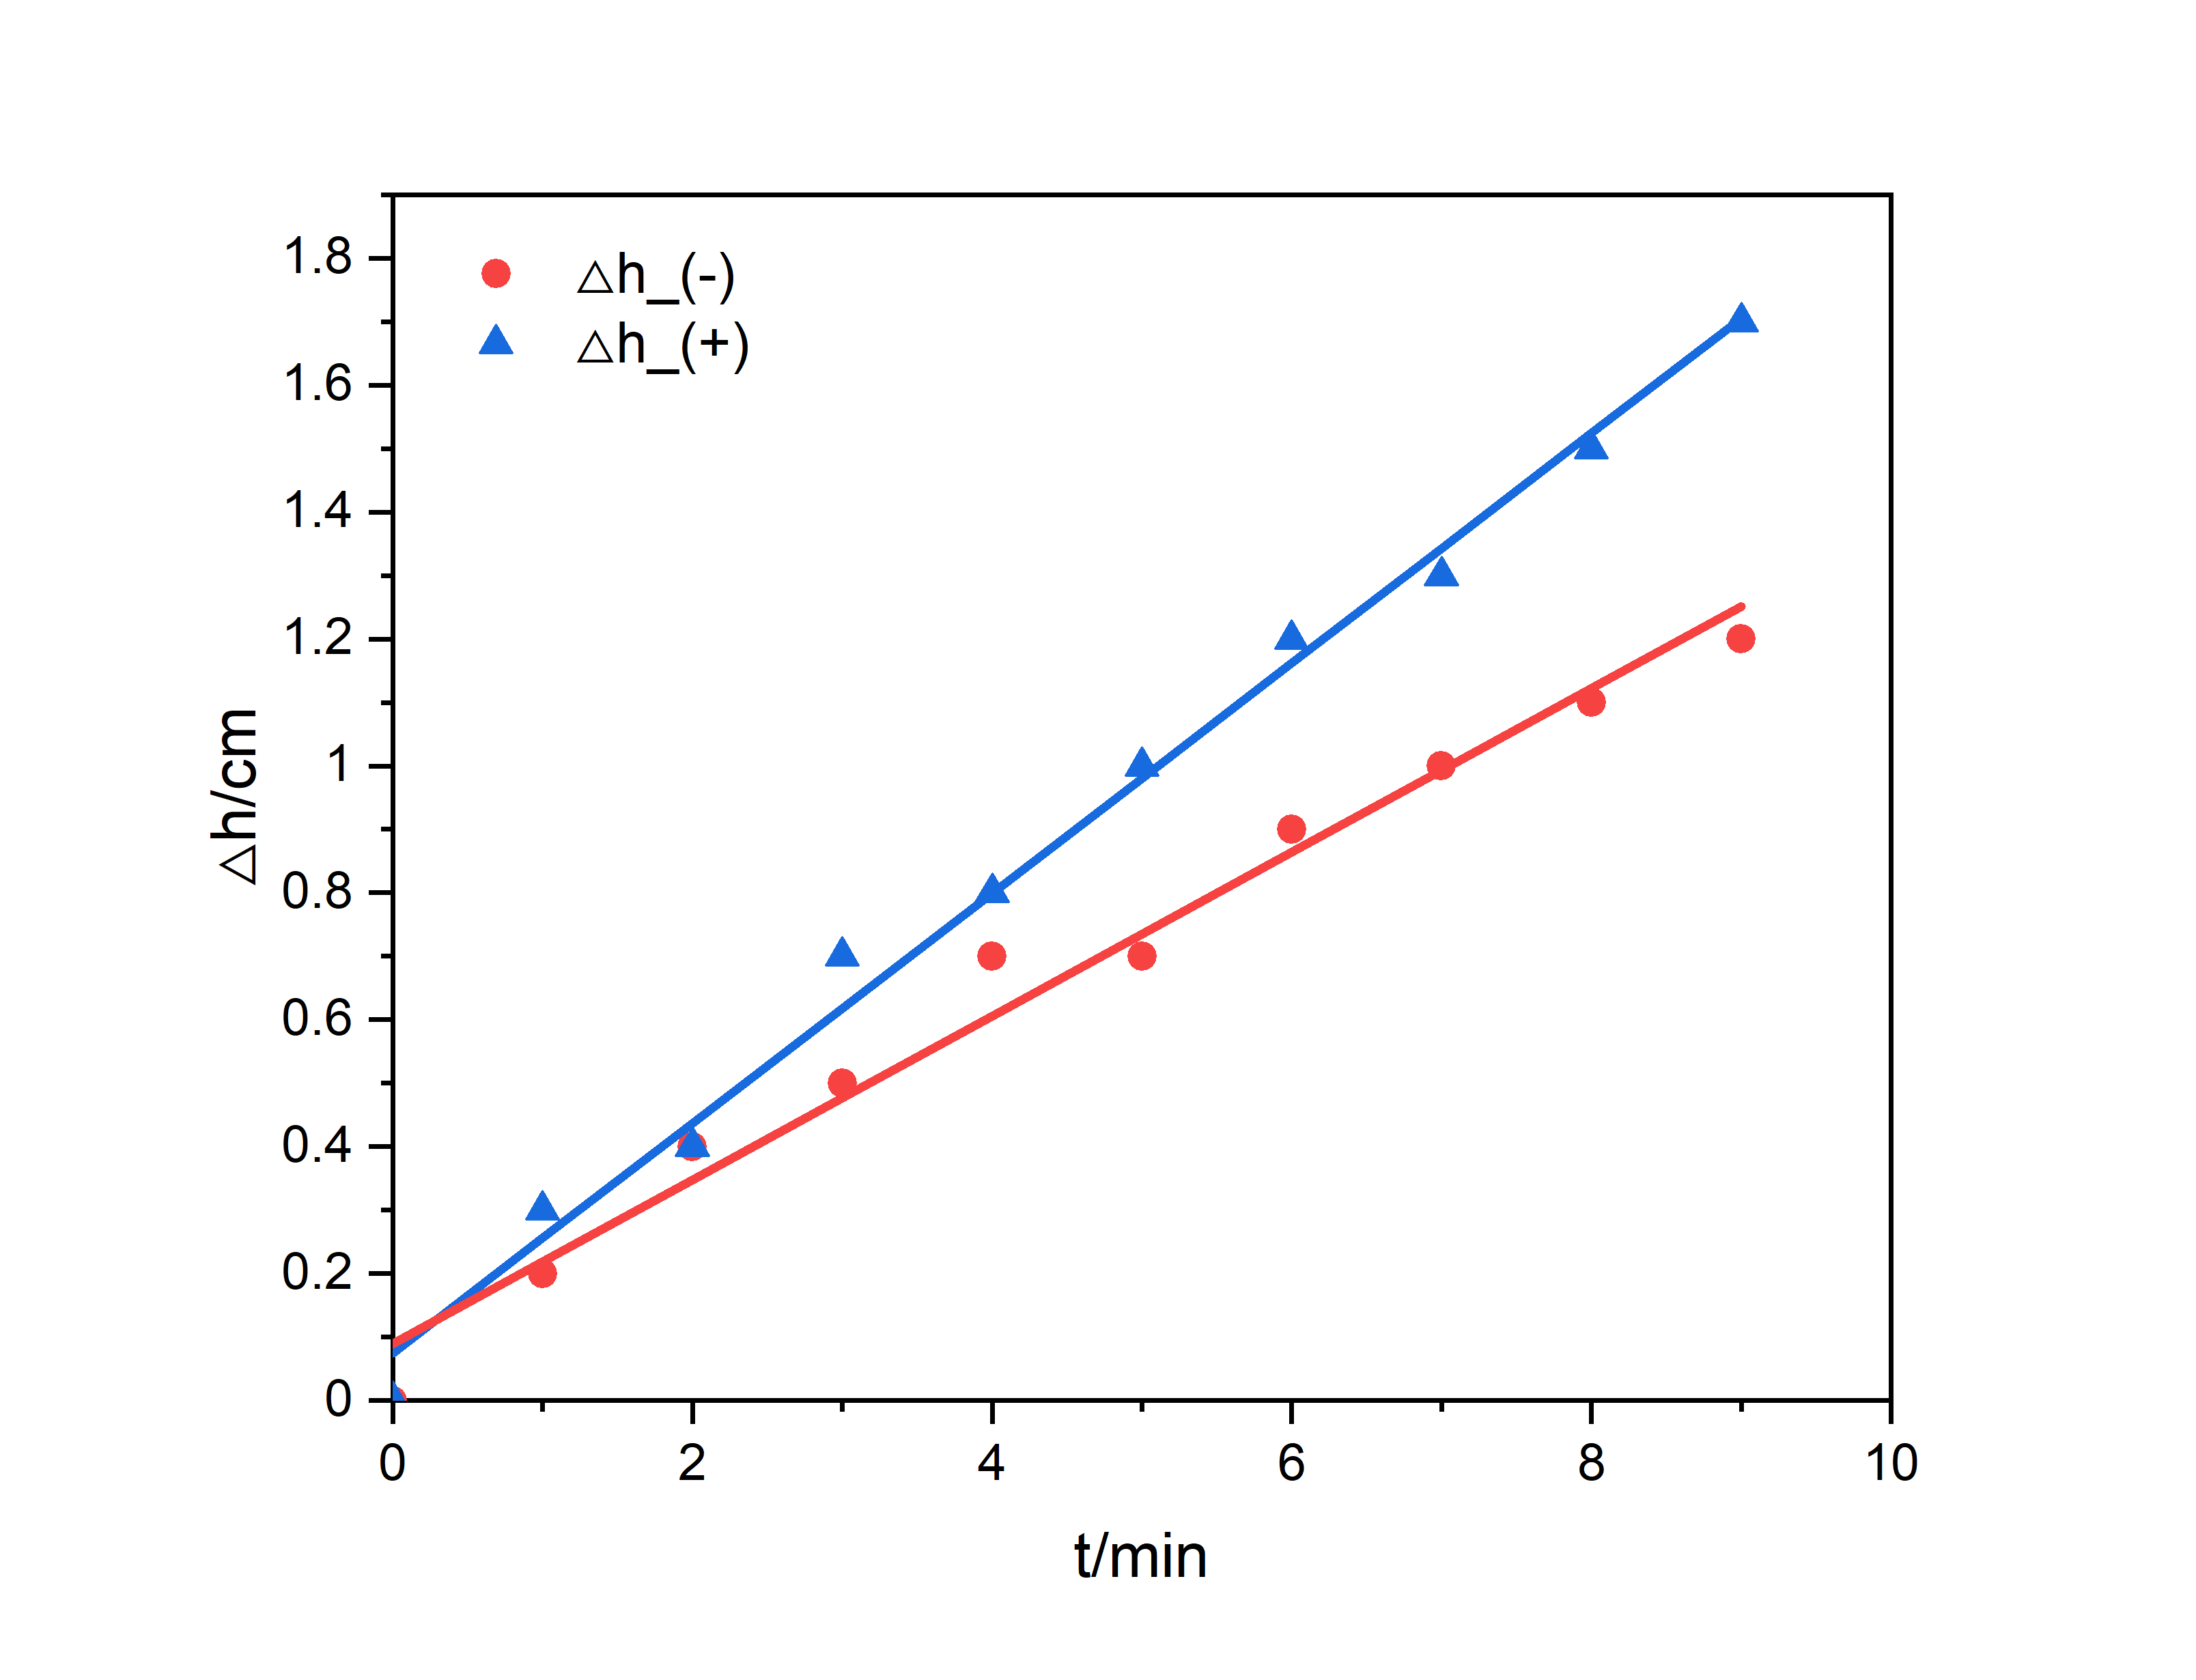
\includegraphics[width = .63\textwidth]{image/Graph3.png}
    \caption{$\Delta h - t$图}\label{7}
\end{figure}

得到
$$
\Delta h_{(-)} =(0.129 \pm 0.006) t + 0.089 \pm 0.034 \quad R^2=0.978 
$$
$$
\Delta h_{(+)} =(0.181 \pm 0.005) t + 0.075 \pm 0.029 \quad R^2=0.991 
$$

在电泳过程中,正负极均出现细密的气泡。由于氢氧化铁溶胶粒子带正电,会向负极迁移,
因此正极界面下降,负极界面上升,在负极一侧逐渐出现絮状沉淀。

由于界面清晰度的原因,负极界面较为模糊,因此数据线性程度不佳,$R^2=0.978$。因此后续我们
采用正极的线性回归数据进行计算。电泳实验中的界面迁移速度可作为胶粒的电迁移速度,因此 $\nu = 0.181 \pm 0.005 {\rm cm \cdot min^{-1}}$

$\rm Fe(OH)_3$溶胶 $\zeta$ 电势的计算公式为
$$
    \zeta = \frac{K\pi\eta\nu}{4\pi E \epsilon_r \epsilon_0} =  \frac{\eta\nu l}{\varphi \varepsilon_r \varepsilon_0}  
$$

其中 $K$ 为粒子形状常数,对于 $\rm Fe(OH)_3$ 为 4,$\eta$ 为介质粘度,$\nu$ 为胶体运动速度,$\varphi$ 为电极间电势差。
查阅文献可得\cite{Weast1988CRC},在 $\rm 20 \degree C$,100 kPa 时,水的粘度系数为 $\eta$ = 1.0016 mPa · s,水的
相对介电常数为 $\varepsilon_r$  = 80.223。
因此可以计算得到

$$
    \zeta = \frac{\eta\nu l}{\varphi \varepsilon_r \varepsilon_0} = {\rm \frac{1.0016\ mPa \cdot s \cdot 0.181\ cm \cdot min^{-1} \cdot 22.84\ cm}{103\ V \cdot 80.223 \cdot 8.8542 \cdot 10^{-12}\ F/m} = 0.09432\ V}
$$
$$
    \sigma_\zeta = \zeta \sqrt{(\frac{\sigma_\nu}{\nu})^2+(\frac{\sigma_l}{ l})^2} = 0.0026\ \rm V
$$
由此可得,测量得到的电动电势为 $94 \pm 3\ \rm mV$

\section{实验结果与讨论}
\subsection{讨论}
\subsubsection{误差分析}

本次实验中,测量得到 $\zeta$ 电势为 $94 \pm 3\ \rm mV$。查阅文献\cite{dianyong},可以得到理想条件下电泳法测得的 $\zeta$ 电势应为
43.0 mV 左右。因此本次实验存在较大的误差。

误差的主要来源为滴加辅助液的速率过快,导致界面清晰度较差,难以分辨正负极界面导致无法准确读数。此外,第二次测量吸出一定量辅助液-胶体混合物
这对胶体的量产生影响,第一次测定已经对溶胶进行了部分电解,负极已经产生了一些絮状沉淀。即使交换正负极也会对测量产生不可忽略的影响。
另外根据文献中的讨论可知\cite{dianyong},溶液的浓度,电解的 pH 值,溶胶的电导率均会对胶体的 $\zeta$ 电势产生影响,因此在特定的温度、浓度与 pH 值等条件下
才能准确地反应测量 $\zeta$ 电势的误差。

\subsubsection{聚沉原因}

在第一次测定前,我们将尿素加入溶胶中来提高界面的清晰度,不料在加入尿素之后却发生了聚沉。经过分析讨论,产生聚沉可能有以下原因:仪器未清洗足够干净引入了电解质,使得胶体聚沉;加入尿素的过程中引入了杂质导致聚沉;
在转移的过程中发生震荡等引起溶胶聚沉;该组同学制备溶胶不稳定。

\subsubsection{改进方案}

本次实验中透析法纯化 $\rm Fe(OH)_3$ 溶胶消耗了大量的时间,因此可以考虑通过改进实验方案来提高效率。
文献提出了一种使用 1:1 强酸、强碱型离子交换树脂对其纯化的方法,能较好地解决透析法时间过长、操作繁复的问题。\cite{fwq}
具体操作为将混合树脂装入漏斗中,底部加少量玻璃纤维以避免树脂流失,控制
溶胶流速在胶体稳定性不被破坏的范围内,反复倒入溶胶至溶胶电导率达到电泳实验要求.

本次试验的另一大难点为保证电泳法中胶体与辅助液的界面清晰,在实验中采用了加入一定量尿素来提高溶胶的密度,使溶胶和辅助液更好的分层。
另外还可以使用注射器等方法减少液体的流量,避免冲坏界面。


\subsection{结论}

本次实验中,首先通过水解 $\rm FeCl_3$ 制备 $\rm Fe(OH)_3$ 溶胶,然后使用透析法纯化 $\rm Fe(OH)_3$ 溶胶,得到溶胶电导率为 156.9 $\rm \mu S \cdot cm^{-1}$ 的红棕色 $\rm Fe(OH)_3$ 溶胶
。然后使用电泳法实验测定 $\rm Fe(OH)_3$ 溶胶的 $\zeta$ 电势,测量得到的电动电势为 $94 \pm 3\ \rm mV$。实验中产生误差的原因
可能有:界面清晰度较差,第二次测量吸出了一定量辅助液-胶体混合物,电泳时温度、浓度与 pH 值的影响等等。

\nocite{*}
\bibliography{reference}
\end{document}
